\documentclass[11pt,a4paper]{article}

\usepackage[margin=2.5cm]{geometry}
\usepackage[T1]{fontenc}
\usepackage[utf8]{inputenc}
\usepackage{lmodern}
\usepackage{microtype}
\usepackage{booktabs}
\usepackage{tabularx}
\usepackage{array}
\usepackage{enumitem}
\usepackage{xcolor}
\usepackage{graphicx}
\usepackage{tikz}
\usetikzlibrary{positioning,arrows.meta,calc}
\usepackage[hidelinks]{hyperref}
\usepackage{url}
\usepackage{placeins}

\setlength{\parskip}{0.5em}
\setlength{\parindent}{0pt}
\renewcommand{\arraystretch}{1.15}

% Red inline markers for things still to fill in. Delete before submitting.

\title{Aspect-Level Sentiment Analysis of Hotel Reviews\\[2pt]
\large MAAI 902 Natural Language Processing \& LLMs --- Assessment Task 2: NLP Solution Design}
\author{Karthik Krishna (Student ID: 1697286)\\
Repository: \url{https://github.com/kk917/hotel-review-aspect-sentiment}}
\date{23 October 2026}

\begin{document}
\maketitle

%--------------------------------------------------------------------
\section{Introduction and problem definition}

A star rating does not tell a hotel manager what to fix. This project builds and tests an NLP pipeline that reports sentiment per aspect (cleanliness, staff, location, room, food, value, noise and facilities) from free-text hotel reviews, and it targets the cases where simple methods fail: negation, contrast, and several aspects in one comment.

\textbf{The problem.} Hotel managers receive a steady stream of online reviews. Today they use the overall score and read comments by hand, and neither works at scale. A score is one number for a stay that went well in some ways and badly in others, while the time needed to read every comment grows with each review, so recurring problems are found late. Review-level sentiment does not solve this, because one label per review hides the mixed opinions a manager needs. Here a review-level classifier reaches only macro F1 0.603, and even a perfect one would still give one label per review.

\textbf{Why the hard cases matter.} Three comments from the data show the problem:
\begin{itemize}[nosep]
  \item ``The room was excellent, but the staff were rude at check in.'' The room is praised and the staff criticised, so no single label is right.
  \item ``The wifi didn't work.'' Negation reverses the meaning of ``work''.
  \item ``Not a clean hotel at all.'' A positive word (``clean'') sits inside a negative statement.
\end{itemize}
A manager needs each aspect scored separately, with negated and contrasted statements read correctly.

\textbf{Why NLP.} Ratings cannot say which aspect upset a guest. Keyword counts find ``staff'' but cannot separate ``staff were lovely'' from ``staff were not lovely'', and a rule that flips polarity after ``not'' breaks on ``not bad'' and on ``clean but noisy''. Language models read the words around a keyword, and aspect-based models also take the aspect as input. To test whether this helps, the project compares a simple baseline with two pretrained transformers on a hand-labelled set that over-represents the hard cases (Section~\ref{sec:pipeline}).

\textbf{Scope.} The solution takes English hotel reviews and, for each comment and each detected aspect, returns positive, negative or neutral. It then builds a per-aspect summary with the source sentences beside every count. Because the eight aspects are keyword-based, an aspect described in unusual words is missed. The system does not detect sarcasm, handle other languages, rank hotels or judge staff, and it writes no free-text summaries. The evidence is about 20,000 Booking.com reviews of European hotels and 201 hand-labelled comment--aspect pairs, so the results show how the approaches compare on this data and say nothing about how they perform on other platforms.

\textbf{Related work.} Early sentiment analysis predicted one overall polarity per text. Work then moved to the aspect level, because one review can express opposing opinions about different aspects \cite{pontiki2014}. SemEval-2014 Task 4 provided shared benchmarks: manually annotated restaurant and laptop reviews, a common evaluation procedure, and 163 submissions from 32 teams \cite{pontiki2014}. A recent survey \cite{zhang2022} organises ABSA by the sentiment elements involved (aspect term, aspect category, opinion term and polarity). It reports that pretrained language models such as BERT and RoBERTa raised performance, and that models usually assume training and test data come from the same distribution. A systematic review of 727 studies \cite{hua2024} finds that ABSA research relies on a narrow set of domains and datasets, which limits how far results generalise. Recent work moves towards instruction-tuned and large language models: InstructABSA \cite{scaria2024} beats earlier methods on SemEval benchmarks, while a broad evaluation \cite{zhang2024} finds that large language models do well with few examples but struggle with complex, structured sentiment tasks. In the survey's terms, this project does aspect sentiment classification for given aspect categories, with a keyword lexicon supplying the aspect and a pretrained model predicting its polarity. The models are used as released, so the project tests how they transfer to hotel reviews without punctuation. It does not fine-tune or prompt a large language model (Section~\ref{sec:pipeline}). Its contribution is a practical comparison on this domain and text type, with an evaluation built around negation, contrast and multi-aspect comments; it proposes no new method.

%--------------------------------------------------------------------
\section{Data considerations and pre-processing}\label{sec:data}

The project uses a random sample of 20,000 reviews from the Kaggle dataset ``515K Hotel Reviews Data in Europe'' \cite{liu515k}, which holds about 515,000 reviews of 1,493 European hotels scraped from Booking.com and is published under the CC0: Public Domain licence. The reviews date from August 2015 to August 2017. Three columns are used: \texttt{Positive\_Review}, \texttt{Negative\_Review} and \texttt{Reviewer\_Score}. After removing duplicates, 19,716 reviews remain.

\textbf{Why this dataset.} Booking.com asks reviewers to write in two boxes, one for what they liked and one for what they disliked, which gives a free but noisy sentiment label for each comment. The text also keeps capitals and words such as ``not'' and ``but'', which the hard cases depend on. An earlier candidate, a TripAdvisor corpus, was rejected after inspection because its text was lower-cased and stripped of stop words, which removes negation cues.

\textbf{Data quality and limits.}
\begin{itemize}[nosep]
  \item All punctuation was stripped by the dataset creators, so sentence boundaries cannot be found and each text box is treated as one short comment (33,236 comments from 19,716 reviews). Rules restored contractions such as ``didn t'' to ``didn't'', so negations stay recognisable.
  \item Reviewers sort their own remarks into the two boxes, so a model trained here may do worse on free-form reviews.
  \item The data covers European hotels only, comes from self-selected reviewers, is scraped, and is mostly English. Scores skew high: 64.6\% of sampled reviews score 8 or higher and 36.3\% score 10. Most reviews are short: the median is 22 words and 79.9\% have fewer than 50.
\end{itemize}

\textbf{Pre-processing.} Cleaning is light: whitespace and links are removed, the placeholders ``No Positive'' and ``No Negative'' become empty, and case and negations are kept. A keyword lexicon tags each comment with up to eight aspects and finds at least one in 85.5\% of comments. Three keyword flags mark hard cases: negation (29.5\% of comments), contrast words such as ``but'' (13.5\%) and several aspects in one comment (49.4\%). The baseline uses TF-IDF with one- and two-word features, and the transformers use their own sub-word representations.

\textbf{Evaluation set.} The box a comment came from is only a weak label, so a hand-checked set was built at aspect level. It has 201 (comment, aspect) pairs in four groups sampled at about 50 pairs each (contrast, negation, multi-aspect and plain); after labelling, group sizes range from 35 to 70. The originating box was hidden. Each pair has a sentiment toward its aspect (positive 94, negative 81, neutral 18, not applicable 8) and a difficulty type, with ``not applicable'' marking keyword false alarms, 4\% of pairs. A language model drafted the labels, and the author then reviewed every row and changed one sentiment label; the draft is kept in frozen columns. Because the reviewer saw the draft, the 99.5\% agreement (kappa 0.992) is not independent inter-annotator agreement. The set is small and stratified by keyword flags, so it does not reflect the natural mix of comments.

%--------------------------------------------------------------------
\section{Pipeline and architecture design}\label{sec:pipeline}

The pipeline turns raw reviews into a per-aspect summary. Reviews are cleaned and split into comments, tagged with aspects, scored for sentiment toward each aspect, and aggregated with their source sentences (Figure~\ref{fig:pipeline}).

\begin{figure}[htb]
\centering
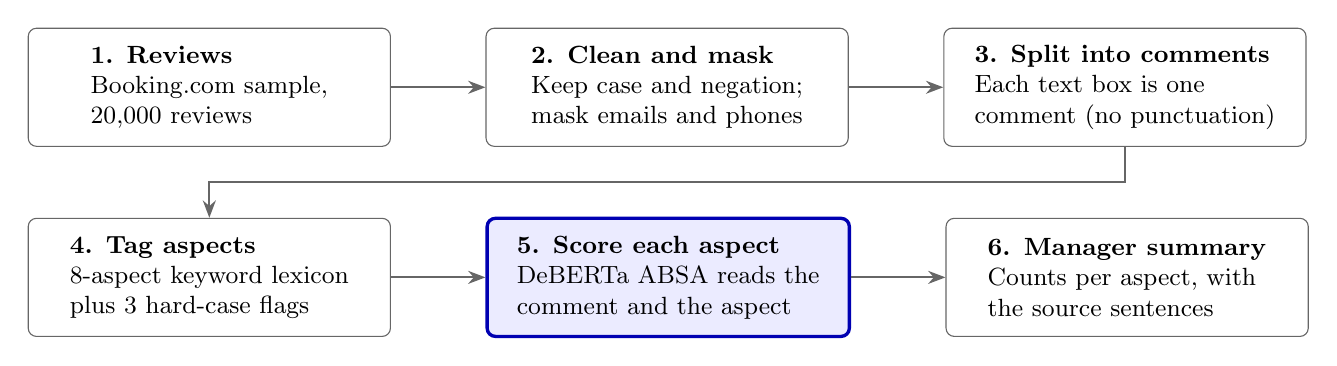
\begin{tikzpicture}[
  node distance=9mm and 12mm,
  box/.style={draw=black!60, rounded corners=3pt, minimum width=4.6cm, minimum height=1.5cm,
              align=left, font=\small, inner sep=5pt},
  main/.style={box, draw=blue!70!black, fill=blue!8, very thick},
  arr/.style={-{Stealth[length=2.2mm]}, black!60, thick}
]
  \node[box] (s1) {\textbf{1. Reviews}\\Booking.com sample,\\20,000 reviews};
  \node[box, right=of s1] (s2) {\textbf{2. Clean and mask}\\Keep case and negation;\\mask emails and phones};
  \node[box, right=of s2] (s3) {\textbf{3. Split into comments}\\Each text box is one\\comment (no punctuation)};
  \node[box, below=of s1] (s4) {\textbf{4. Tag aspects}\\8-aspect keyword lexicon\\plus 3 hard-case flags};
  \node[main, right=of s4] (s5) {\textbf{5. Score each aspect}\\DeBERTa ABSA reads the\\comment and the aspect};
  \node[box, right=of s5] (s6) {\textbf{6. Manager summary}\\Counts per aspect, with\\the source sentences};
  \draw[arr] (s1) -- (s2);
  \draw[arr] (s2) -- (s3);
  \draw[arr] (s3.south) -- ++(0,-0.45) -| (s4.north);
  \draw[arr] (s4) -- (s5);
  \draw[arr] (s5) -- (s6);
\end{tikzpicture}
\caption{The pipeline. Step 5 (highlighted) is the only step that sees the aspect it is judging. Five models are compared at this step on the same 201 hand-labelled pairs.}
\label{fig:pipeline}
\end{figure}

\textbf{Model choices.} Five predictors are compared on the same labelled pairs to test one question: does telling the model the aspect help with negation, contrast and multi-aspect comments?
\begin{itemize}[nosep]
  \item \emph{Majority class} is the floor.
  \item \emph{TF-IDF + logistic regression} is the standard baseline. It reads the whole comment and ignores the aspect. It is trained on 29,735 weak-labelled comments (labelled by their box), excluding every review in the evaluation set. Settings: one- and two-word features, minimum document frequency 2, sublinear term frequency, balanced class weights.
  \item \emph{RoBERTa sentiment} \cite{cardiff} is a pretrained transformer that reads context, so it can in principle handle ``not bad''. It is aspect-blind and gives one label per comment.
  \item \emph{DeBERTa ABSA} \cite{yangheng} is a pretrained aspect-based model. It reads the pair (comment, aspect), so ``the room was excellent but the staff were rude'' can score room and staff differently, which is why the design uses it for multi-aspect and contrast cases.
  \item \emph{Box label} returns the box a comment came from. A real system would not have this information, so it is included only as a reference ceiling for weak labels.
\end{itemize}
A prompted large language model was considered but not evaluated: a language model drafted the labels, so the comparison would be partly circular.

\textbf{Tuning.} The transformers are used as released, with no fine-tuning or hyperparameter search, because the evaluation set is too small (201 rows) to tune on without overfitting. Weak-label splits are made by review, so comments from one review never appear in both training and test sets.

\textbf{Evaluation design.} Models are scored on the 193 labelled pairs with a real sentiment (the 8 not-applicable pairs are excluded). Metrics are accuracy with a 95\% bootstrap interval, three-class macro F1, and error counts per group. Macro F1 needs care: TF-IDF and the box label can only answer positive or negative, so they score zero on the 18 neutral pairs, which caps their macro F1 near 0.6. Accuracy is therefore the fairer headline.

\textbf{Results.} Two earlier baselines frame the task. A review-level TF-IDF classifier reaches macro F1 0.603 but says nothing about aspects. A comment-level classifier predicting the box reaches 0.943, a figure that measures how well it recovers the box and says nothing about whether it understands aspects. On the hand-labelled pairs, Table~\ref{tab:overall} gives overall results and Table~\ref{tab:errors} gives errors by group.

\begin{table}[htb]
\centering
\caption{Overall results on the 193 scored pairs.}
\label{tab:overall}
\begin{tabular}{lcc}
\toprule
Model & Accuracy (95\% interval) & Macro F1 (3-class) \\
\midrule
Majority class & 0.42 to 0.55 & 0.218 \\
Box label (reference) & 0.82 to 0.91 & 0.604 \\
TF-IDF + LogReg & 0.80 to 0.90 & 0.594 \\
RoBERTa (aspect-blind) & 0.65 to 0.77 & 0.575 \\
DeBERTa ABSA (aspect-aware) & 0.76 to 0.87 & 0.627 \\
\bottomrule
\end{tabular}
\end{table}

\begin{table}[htb]
\centering
\caption{Error counts by difficulty group (lower is better).}
\label{tab:errors}
\begin{tabular}{lccccc}
\toprule
Model & Contrast & Negation & Multi-aspect & Plain & Total of 193 \\
\midrule
TF-IDF + LogReg & 20 & 4 & 2 & 3 & 29 \\
RoBERTa (aspect-blind) & 22 & 12 & 1 & 20 & 55 \\
DeBERTa ABSA (aspect-aware) & 15 & 9 & 3 & 8 & 35 \\
\bottomrule
\end{tabular}
\end{table}

\textbf{Discussion.} These results give five findings.

First, the aspect-aware model beats the aspect-blind one, so telling the model the aspect helps. Their accuracy intervals barely touch (0.65 to 0.77 and 0.76 to 0.87), and on the paired comparison DeBERTa was right and RoBERTa wrong on 30 pairs, and the reverse on 10.

Second, a cheap model trained on about 30,000 weak-labelled in-domain comments matches DeBERTa overall (the intervals overlap heavily, so this is a tie) and beats RoBERTa, having learned this dataset's style.

Third, contrast is the hardest group for every model, with accuracy of 0.41 to 0.59 against 0.63 to 0.99 elsewhere. DeBERTa is best (0.59, macro F1 0.52, against 0.36 for RoBERTa and 0.38 for TF-IDF). Many of these errors involve neutral labels: 12 of DeBERTa's 15 contrast errors, 13 of TF-IDF's 20 and 11 of RoBERTa's 22. The human called these pairs neutral, usually because the comment is mixed (``Rooms are small but typical for Paris They were very well appointed however''). The scheme has no mixed class, so a model that picks a side is marked wrong, and TF-IDF cannot answer neutral at all. Part of the difficulty with contrast is therefore real and part is a limit of three-class labels.

Fourth, negation is the second weak spot. TF-IDF's four negation errors do not show that it understands negation: most negation pairs are negative, and a bag of words that maps ``not'' to negative scores well without handling scope. The aspect-aware model does not solve scope either. All three models called the value of ``Great location Club prices for not a club experience'' positive, and DeBERTa labelled ``Pillows and bed are not comfortable at all'' neutral. RoBERTa's main weakness is mild complaints: of its 55 errors, 28 are negative pairs it called neutral, such as ``the bedroom was a bit small'' and ``Tiny room for 150 EUR per night''. This is probably because it was trained on tweets, not hotel complaints.

Fifth, all models made few errors on multi-aspect pairs (1 to 3), and DeBERTa shows no advantage there. A text box holds either praise or complaint, so the aspects in one comment usually share a sentiment, and the sample has few comments where aspects truly disagree. With 35 to 70 pairs per group, group-level differences are noisy and indicative only.

%--------------------------------------------------------------------
\section{Tools, frameworks and platforms}\label{sec:tools}

The stack is small and open source, so the work can be rerun in a free Colab session.

\begin{table}[htb]
\centering
\caption{Tools and the reason each was chosen.}
\label{tab:tools}
\small
\begin{tabularx}{\textwidth}{>{\raggedright\arraybackslash}p{2.7cm}>{\raggedright\arraybackslash}X>{\raggedright\arraybackslash}X}
\toprule
Tool & Role & Why chosen \\
\midrule
Hugging Face Transformers & Runs the pretrained RoBERTa and DeBERTa models through one interface & Gives both models in a few lines; training from scratch is not feasible here \\
scikit-learn & TF-IDF, logistic regression, metrics, kappa, splits by review & Standard and fast; a simple baseline shows what transformers add \\
pandas & Loading, sampling and cleaning the CSV; holding comments and labels & The sample fits in memory, so no database is needed \\
spaCy & Rule-based sentence splitting when installed (regex fallback) & A light sentencizer suffices; the text has no punctuation \\
Gradio & The demo app: paste reviews, see the summary and evidence & One function gives a shareable interface; Streamlit or Flask need more code \\
Colab and Drive & Notebooks and free GPU inference & No local setup. The notebooks also run locally \\
GitHub & Version control and delivery of commented code and README & Required by the brief and records the history \\
\bottomrule
\end{tabularx}
\end{table}

LangChain was left out because the pipeline is a fixed sequence of functions, and a hosted LLM API was left out so that results can be reproduced without a key or cost.

%--------------------------------------------------------------------
\section{Ethical and responsible AI considerations}\label{sec:ethics}

The main risks come from the people behind the text and from over-trusting a small, partly automated evaluation. Each mitigation is marked as built or proposed.

\begin{enumerate}[nosep]
  \item \textbf{Reviewer privacy.} Reviews can contain names, phone numbers, emails or room numbers. \emph{Built:} the demo masks emails, phone numbers and links before analysis or display, and the dataset is not redistributed. \emph{Proposed:} a named-entity model to mask personal names, which patterns cannot find, and storing only masked text.
  \item \textbf{Fake or incentivised reviews.} Scraped reviews may include paid or fabricated ones, which distort the scores a manager sees. \emph{Built:} exact duplicates are removed. \emph{Proposed:} detecting bursts of near-identical reviews, and showing review counts beside every score.
  \item \textbf{Language and dialect bias.} The data is mostly English, from European hotels, written by reviewers who chose to write. Performance may be worse for non-native English, slang or very short comments. \emph{Built:} results are reported by difficulty group with intervals that show how little 193 rows can prove. \emph{Proposed:} accuracy by review length and language before any deployment.
  \item \textbf{Hallucination and over-claiming.} A language model summary could invent complaints. \emph{Built:} the demo writes no free text, and every count links to its source sentences, so a manager can verify it. The aspect tagger has a known false-alarm rate (4\% of labelled pairs), which is why evidence is shown with every score.
  \item \textbf{Unfair consequences for named staff.} A negative comment about a person could be used to discipline them on weak evidence. \emph{Built:} results are aggregated by aspect (for example ``staff''), and nothing is grouped by person. Source sentences are shown, so a name in a comment would still appear until name masking (item 1) is added. \emph{Proposed:} human review before any personnel decision, and wording that scores describe guest perception.
  \item \textbf{Weak and AI-assisted labels.} Training labels come from the box a comment was written in, which is noisy. A language model drafted the evaluation labels before a human checked them. A reviewer who sees a draft may anchor on it, so the 99.5\% agreement is not independent evidence of quality. \emph{Built:} the draft is kept in frozen columns, the process is disclosed here, and no LLM is scored. \emph{Proposed:} a second annotator working blind.
  \item \textbf{Data provenance.} The data was scraped from a booking site and uploaded by a third party, so reviewers did not consent to this use. The Kaggle licence (CC0) comes from the uploader and cannot grant rights over the Booking.com content or the reviewers' text. \emph{Built:} the data is used for coursework only, is not redistributed and is cited.
\end{enumerate}

Overall, the system should be a triage tool that shows a manager where to look, with the evidence, and never an automatic judge of hotels or people.

%--------------------------------------------------------------------
\section{Expected output, value proposition and conclusion}\label{sec:output}

The prototype gives a manager a ranked list of aspects, worst first, with the sentences behind every number. Figure~\ref{fig:demo} comes from the demo run on four short example reviews; it illustrates the output and is not an evaluation.

\begin{figure}[!htbp]
\centering
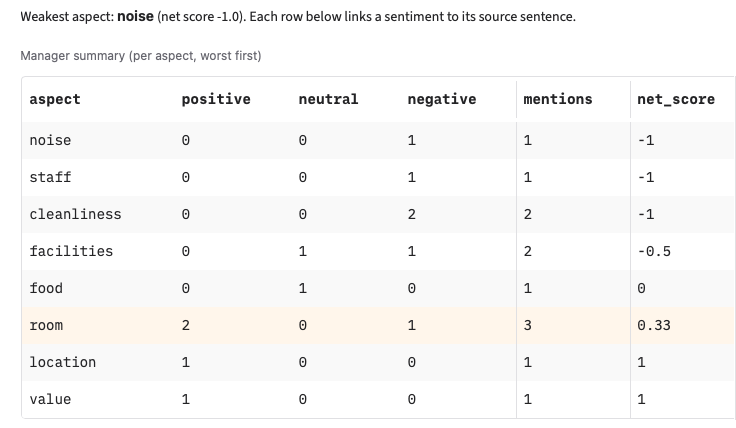
\includegraphics[width=0.74\textwidth]{demo_summary.png}\\[6pt]
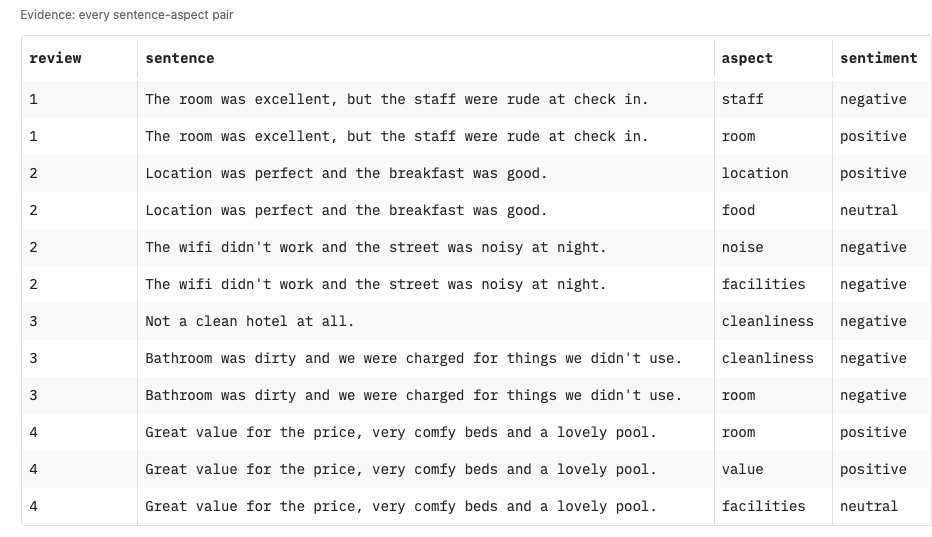
\includegraphics[width=0.94\textwidth]{demo_evidence.png}
\caption{The Gradio demo on four example reviews. Top: the manager summary, worst aspect first (net score = (positive $-$ negative) / mentions). Bottom: the evidence table linking every sentiment to its source sentence.}
\label{fig:demo}
\end{figure}


The evidence table lets a manager check any count. The aspect-aware model also separates opinions that one label would merge: for ``The room was excellent, but the staff were rude'' it returns room positive and staff negative, whereas the aspect-blind RoBERTa returns positive for both.

\textbf{Value.} The tool helps a manager decide where to look first. Instead of reading every comment, they see which aspects attract the most complaints and can open the exact sentences, and recurring problems such as noise or cleanliness show up as a pattern across reviews. Each score is traceable and nothing is generated as free text, so the output can be checked. This report did not measure time saved or business impact, which remain hypotheses to test with real managers.

\textbf{Limitations.} The demo also shows the system's weaknesses. The model labelled ``the breakfast was good'' and ``a lovely pool'' as neutral, and ``the wifi didn't work'' as neutral in one test. The keyword tagger counted ``Bathroom was dirty'' under room as well as cleanliness, and it missed cleanliness in ``Not the cleanest hotel''. These match Section~\ref{sec:pipeline}: a DeBERTa accuracy interval of 0.76 to 0.87, a weak showing on contrast, and a lexicon that limits which aspects are found. The results come from one dataset, and one person checked the AI-drafted labels.

\textbf{Future work.} The most useful next steps are:
\begin{itemize}[nosep]
  \item fine-tune the aspect-aware model on this domain;
  \item replace the keyword tagger with a learned aspect extractor;
  \item mask personal names with a named-entity model;
  \item add a second, blind annotator and a ``mixed'' label;
  \item test a prompted language model and the tool with real managers.
\end{itemize}

\textbf{Conclusion.} Review-level scores hide what managers need to know, and a pipeline that tags aspects and scores each one separately recovers more of it. In these experiments the aspect-aware transformer was more accurate than the aspect-blind one and made fewer errors on contrast, while a simple in-domain baseline stayed competitive overall. Aspect-level analysis is feasible and checkable with modest tools, but contrast and negation remain hard, and a larger, independently labelled evaluation is needed before anyone relies on it.

%--------------------------------------------------------------------
\FloatBarrier
\begin{thebibliography}{9}
\bibitem{pontiki2014}
Pontiki, M., Galanis, D., Pavlopoulos, J., Papageorgiou, H., Androutsopoulos, I.\ and Manandhar, S.\ (2014)
`SemEval-2014 Task 4: Aspect Based Sentiment Analysis',
\emph{Proceedings of the 8th International Workshop on Semantic Evaluation (SemEval 2014)}, Dublin, Ireland, pp.\ 27--35.
Available at: \url{https://aclanthology.org/S14-2004/}

\bibitem{zhang2022}
Zhang, W., Li, X., Deng, Y., Bing, L.\ and Lam, W.\ (2022) `A Survey on Aspect-Based Sentiment Analysis: Tasks, Methods, and Challenges', \emph{arXiv preprint} arXiv:2203.01054.
Available at: \url{https://arxiv.org/abs/2203.01054} (Accessed: 23 October 2026).

\bibitem{hua2024}
Hua, Y.\ C., Denny, P., Wicker, J.\ and Taskova, K.\ (2024) `A systematic review of aspect-based sentiment analysis: domains, methods, and trends', \emph{Artificial Intelligence Review}, 57, article 296.
Available at: \url{https://link.springer.com/article/10.1007/s10462-024-10906-z} (Accessed: 25 October 2026).

\bibitem{scaria2024}
Scaria, K., Gupta, H., Goyal, S., Sawant, S., Mishra, S.\ and Baral, C.\ (2024) `InstructABSA: Instruction Learning for Aspect Based Sentiment Analysis', \emph{Proceedings of NAACL 2024 (Short Papers)}, Mexico City, pp.\ 720--736.
Available at: \url{https://aclanthology.org/2024.naacl-short.63} (Accessed: 25 October 2026).

\bibitem{zhang2024}
Zhang, W., Deng, Y., Liu, B., Pan, S.\ and Bing, L.\ (2024) `Sentiment Analysis in the Era of Large Language Models: A Reality Check', \emph{Findings of NAACL 2024}, pp.\ 3881--3906.
Available at: \url{https://aclanthology.org/2024.findings-naacl.246} (Accessed: 25 October 2026).

\bibitem{liu515k}
jiashenliu (n.d.) \emph{515K Hotel Reviews Data in Europe} [Dataset]. Kaggle.
Available at: \url{https://www.kaggle.com/datasets/jiashenliu/515k-hotel-reviews-data-in-europe} (Accessed: 23 October 2026).

\bibitem{cardiff}
cardiffnlp (n.d.) \emph{twitter-roberta-base-sentiment-latest} [Model]. Hugging Face.
Available at: \url{https://huggingface.co/cardiffnlp/twitter-roberta-base-sentiment-latest} (Accessed: 23 October 2026).

\bibitem{yangheng}
yangheng (n.d.) \emph{deberta-v3-base-absa-v1.1} [Model]. Hugging Face.
Available at: \url{https://huggingface.co/yangheng/deberta-v3-base-absa-v1.1} (Accessed: 23 October 2026).
\end{thebibliography}

\end{document}
